\chapter{概览}
\label{cap:overview}
    我们模型的主要目标,就是拿到神经网络的结构,预测该神经网络在特定硬件环境下的运行时间。特别地,我们的模型针对TensorFlow框架,也就是说,所有性能数据全部来源于TensorFlow,因此,我们的预测结果在其他深度学习框架中不一定能够得到较好的预测结果。另一方面,我们模型主要针对CNN进行设计,能够在现有的广泛使用的CNN网络上有比较好的预测结果,如AlexNet\cite{alexnet}等。我们将工作限制在单机上,对仅CPU、1个GPU、2个GPU、4个GPU环境进行测试建模,得到较为满意的预测性能。
    
\section{模型配置}
    模型的输入部分包括网络的结构或网络对应的数据流图、各个计算模块的参数、运行的硬件平台,共三部分。
    
    网络结构在执行过程中,会先转换为数据流图的形式,这一部分对深度神经网络进行主要的定义。而由于数据流图对输入的形状、维度等没有严格的限制,如图\ref{fig:dag_same}所示。因此,输入部分需要对输入的形状进行预先的定义,以便于之后模型进行模拟调度以及性能预测。
    
    另外,输入需要提供运行的硬件环境,如CPU数量、CPU核心数量、内存大小、GPU型号、GPU显存大小、GPU的数量等。以便模型针对不同硬件环境进行调整。限于资源有限,我们只实现了几个固定环境中的性能模型,因此,现有模型的硬件环境配置只能够调整为固定的几种配置,具体见测试部分第\ref{cha:eval}章节。

    \begin{figure}[!htbp]
        \centering
        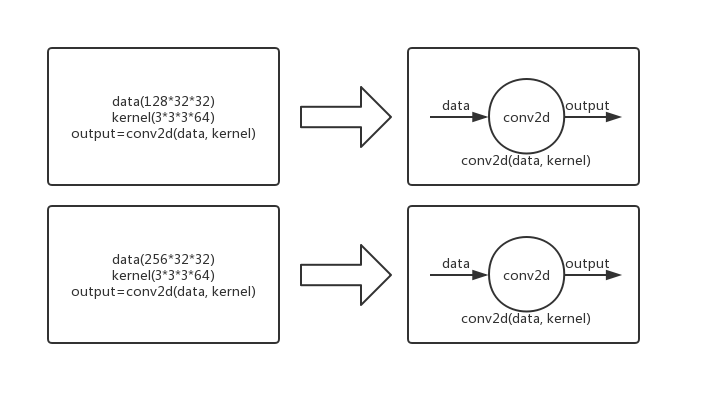
\includegraphics[width=0.8\textwidth]{figures/dag_same.jpg}
        \caption{图中预先定义的两个网络,输入的形状不同,但是生成的数据流图是相同的}
        \label{fig:dag_same}
    \end{figure}
    
\section{模型架构}    
    我们实现的预测模型整体架构如图\ref{fig:arch}所示。主要实现包含两部分,即图中的调度模拟,和性能模型两部分。其中,调度模拟部分根据深度神经网络应用在运行过程中生成的数据流图,模拟预测真实运行情况下每一个操作的运行状况,包括运行的顺序,运行所在设备,运行占用资源等。性能模型部分根据实际Tensorflow中操作运行的时间,建立操作性能模型。得到的结果再提供给调度模拟部分,两部分结合,继而在操作的粒度上,预测在正常的Tensorflow的调度下,深度神经网络应用的运行时间。
    
    \begin{figure}[!htbp]
        \centering
        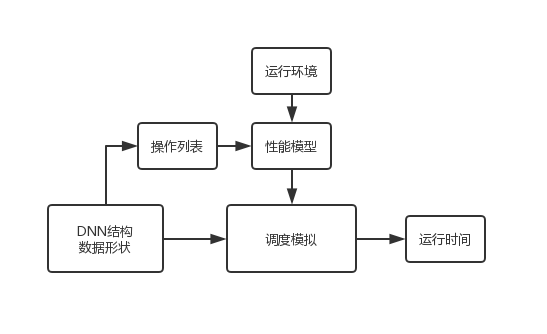
\includegraphics[width=0.8\textwidth]{figures/arch.jpg}
        \caption{预测模型整体架构}
        \label{fig:arch}
    \end{figure}

\subsection{调度模拟}
    TensorFlow中所有的计算任务会被转化为数据流图的形式,其中每个点代表一个计算操作,每一条边表示一组数据。具体到实际运行TensorFlow中,每一个点代表一个计算函数,如矩阵乘法(MatMul)、二维卷积(Conv2D)等,而一条边代表一个张量(tensor)。调度模拟部分的主要工作就是将用户定义的神经网络模型转化为数据流图,并针对数据流图按照tensorflow的方式进行调度。
    
    TensorFlow中,执行计算任务是通过会话(session)的方式进行的,即执行Session.run()命令。在这个过程中,首先进行的是会话的创建,与此同时,将模型转化为数据流图的形式保存。我们的工作主要关注的就是这一步生成的数据流图。而数据流图在创建到运行的过程中,需要经历六个阶段,即图的创建、图的传送、图的剪枝、图的划分、图的二次划分,以及图的运行。下面我将分别对这些部分进行解释。
    
    图的创建,根据用户写入的模型创建数据流图。用户在使用TensorFlow的时候,神经网络是以运算的形式定义的。由于用户的输入为计算任务或数据生成任务,因此,用户的输入均可以直接对应数据流图中的一个子图。以图\ref{fig:dag_mat}中定义的网络为例,用户定义了两个矩阵,即通过random\_normal操作生成两个$ 5000 \times 5000 $ 的服从正态分布的矩阵$ a $和$ b $。之后定义$ c = a \times b $,$ d = b * c $,最终输出为矩阵$ d $。而在创建图的过程中,输入均被映射到数据流图中的一个子图,其中每个子图都按照对应的任务,对应了一个小的数据流图,如图中random\_normal操作被转化成3个节点,random\_normal、mul、add,分别用来生成原始数据,调整标准偏差,调整平均值。再将所有子图进行连接。从另一个角度来看,每个计算任务都被先转化成了一个数据流图,先行生成若干子图,再按照用户定义的数据依赖关系组合,就得到了我们创建的数据流图。
    
    \begin{figure}[!htbp]
        \centering
        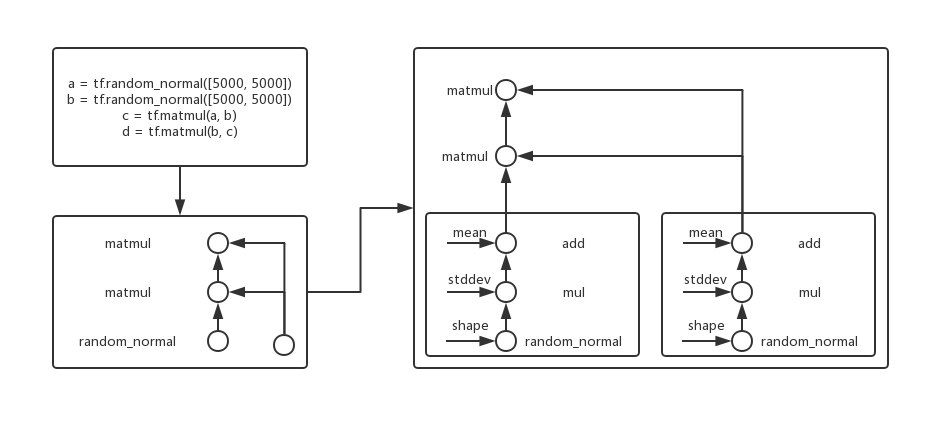
\includegraphics[width=0.8\textwidth]{figures/dag_mat.jpg}
        \caption{数据流图的创建过程}
        \label{fig:dag_mat}
    \end{figure}

    图的传送,主要任务是把已经生成好的数据流图序列化,并传送给计算的主机(master)。这一步把之前生成的图(Graph)转化为图定义(GraphDef),再传送给主机。主机是TensorFlow在运行过程中的概念,这一部分与我们的性能预测模型关系不大,因此不做过多介绍。
    
    图的剪枝,根据给定输入与需求输出得到最小依赖集。主机(master)在得到图定义(GraphDef)后,先进行反序列化转化为原图(Graph),然后根据给定的输入,和需求的输出,对图进行剪枝,具体过程就是进行深度优先搜索(DFS),对图进行标记,从而确定哪些点是得到输出中必要的,并删除其他所有节点和无关的边,将图的规模缩小。
    
    图的划分,把图中的节点分配到不同的机器(worker)上。在Tensorflow中进行多机并行时,需要手动对计算图进行划分,即规定运算所在的机器。在数据并行中,用户需要手动将数据分成若干组,给每一组规定运行的机器。在模型并行中,用户需要规定操作所在的机器。这一步的工作,就是根据用户的输入定义,将图的节点或子图分配到各个机器上。
    
    图的二次划分,把图中节点分配到不同的设备上。机器(worker)根据当前可用的资源,以及用户对操作的约束,将途中的节点分配到不同设备上,如CPU,GPU等。默认情况下,大部分运算操作都会被划分到GPU上。
    
    图的运行,将划分好的节点运行。TensorFlow中执行运算使用StreamExecutor。在图经过两次划分后,对划分好的子图或点进行运行,这一部分TensorFlow会对每个子图启动一个执行器(Executor)实例,用来对这个子图进行运算,StreamExecutor简单来说可以理解成对底层设备的封装,TensorFlow通过StreamExecutor进行执行,可以避免对底层硬件的直接接触。实际运行过程中,如果使用GPU,这里的大部分操作都会被映射为CuBlas函数或CuDNN\cite{cudnn}函数。
    
    调度模拟部分从图的创建开始,进行到图的两次划分为止。由于我们的模型主要运行在单机,因此图的划分这一部分实际均会被划分到同一台机器上。而图的二次划分部分,被放在性能模型部分进行,即对每个操作,根据给定的运行环境,选择不同的模型进行预测。因此,调度模拟部分主要工作就是将用户定义的输入转化为对应的数据流图并剪枝,然后对每个节点调用性能模型。

\subsection{性能模型}
    在卷积神经网络中,通常计算以层的形式进行组织,每一层包含一个或多个并列的操作。以AlexNet在CPU上的执行过程为例,如图\ref{fig:alexnet_timeline}所示。我们可以观察到,运算在时间上明显分层,并且在有的层有明显的并行性。另外,其中明显占用时间的操作有\_FusedConv2D、Conv2DBackPropFilter、Conv2DBackPropInput、MatMul等。
    
    事实上,在AlexNet运行在CPU上时,其中占用运算时间最长的三个操作均与二维卷积相关(前三名分别为对输入求二维卷积梯度(Conv2DBackPropInput)、对卷积核求二维卷积梯度(Conv2DBackPropFilter)、复合二维卷积(\_FusedConv2D)),其次为局部相应归一化(LRN)和矩阵乘法(MatMul)及相应的梯度计算。而无论是更换其他卷积神经网络,或使用GPU,都有相同的结论,即几乎所有时间均消耗在以上几个操作。因此,我们只要针对这三个操作以及其梯度求解进行性能建模,即可比较好的还原卷积神经网络的运行状况。
    
    \begin{figure}[!htbp]
        \centering
        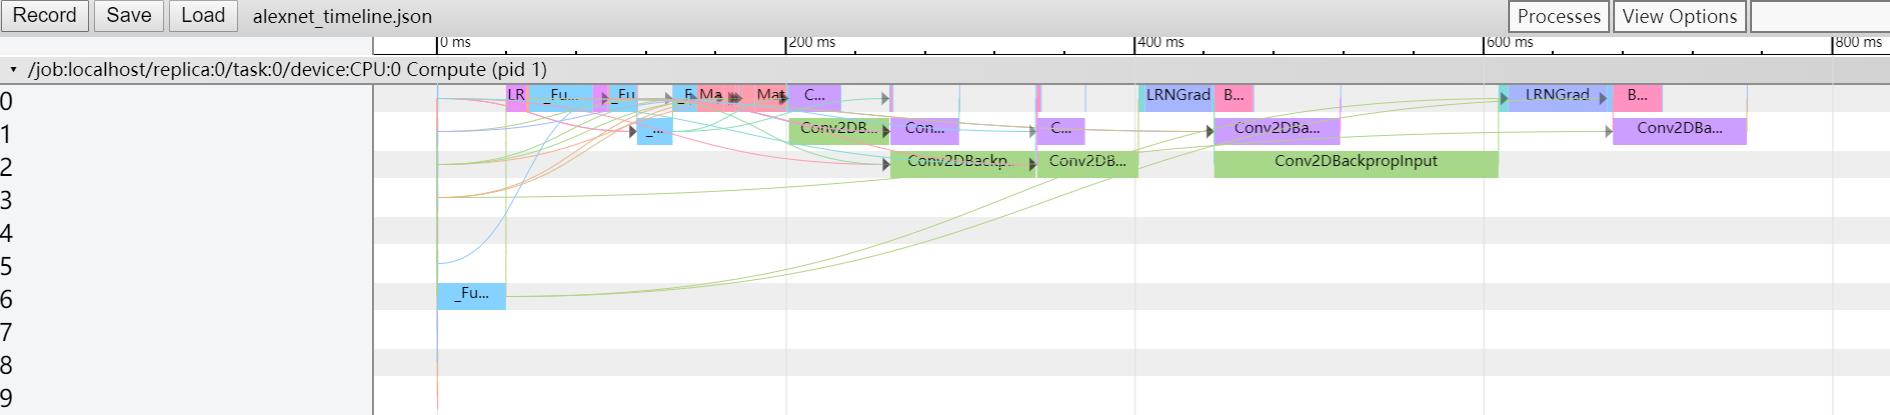
\includegraphics[width=0.8\textwidth]{figures/alexnet_timeline.png}
        \caption{AlexNet在CPU运行的时间线数据}
        \label{fig:alexnet_timeline}
    \end{figure}

\subsubsection{矩阵乘法}
\label{overview:matmul}
    全连接层是卷积神经网络中非常重要的组成部分,通常出现在卷积神经网络的最后,用来统合之前操作得到的局部特征。而全连接层的操作就是二维矩阵的乘法。相比其他操作,全连接层的参数数量要大的多,因此运行时间也会比较长,所以,即使整个网络仅有一个矩阵乘法操作,这一操作也会占用非常可观的运行时间,对矩阵乘法进行性能预测是比较重要的。
    
    矩阵乘法的输入为两个矩阵,即两个二维张量。其中矩阵$ A $的形状为$ M \times P $,矩阵$ B $的形状为$ P \times N $,输出为矩阵$ C = A \times B $,形状为$M \times N$。其中,$ C_{m, n} = \sum_{p=1}^P{a_{m, p} \times b_{p, n}} $。在单线程运行情况下,矩阵乘法的复杂度为$ O( M NP) $。但是,由于数据的局部性,即使$ M \times N \times P $固定,矩阵乘法操作的运行时间也并不固定,因此矩阵乘法的性能建模需要三个参数,即$ M $、$ N $、 $ P $,而不能仅仅将$ M \times N \times P $作为参数。
    
    在TensorFlow中,如果指定使用CPU,系统会使用Eigen\cite{eigen}进行矩阵运算。如果指定使用GPU,系统会使用CuBlas进行运算。因此,我们在实现部分将直接针对CPU和GPU上不同参数下,测量运行时间,继而得到矩阵乘法的性能模型。另外,矩阵乘法部分的梯度计算同样是一个相同规模的矩阵乘法,因此,矩阵乘法的梯度计算不需要单独进行测试,而实际上,在TensorFlow生成的数据流图中,这一计算也直接被生成成为矩阵乘法,不需要再做其他操作了。

\subsubsection{二维卷积}
    二维卷积网络是卷积神经网络的核心运算。通常来说,卷积神经网络中,二维卷积层和池化层(Pooling)是成对出现的,在实际TensorFlow的执行过程中,这两步也是被合并执行,合并统计的。因此,在本文中,我们提到的二维卷积操作即代表合并过的操作,进行建模。
    
    二维卷积操作的输入主要包含三个参数,输入数据(input)、卷积核(filter)、步长(stride)。其中,输入数据是一个四维张量,包括批量大小(batch size)、图片的高度(height)、图片的宽度(width)、图片的通道数量(channel)。批量大小表示一次运算的图片数量,图片的高度宽度定义了图片的尺寸。通道数量表示图片的维度,如灰度图片,通道数为1;RGB图片,通道数为3。而卷积操作对图片进行局部特征提取后,需要多个通道去保存参数,因此会生成较多通道数的中间数据。卷积核也是一个四维张量,包括卷积核的高度(filter\_height)、卷积核的宽度(filter\_width)、输入通道数(in\_channels)、输出通道数(out\_channels)。其中,运算要求卷积核中定义的输入通道数和输入数据中的通道数保持一致,否则运算不能进行。步长是一个四维张量,表示每次点积运算之间横纵坐标的移动距离,即每步移动多少,通常,由于每个图片,每个通道都要进行处理,因此步长只有第二第三个参数有取值,第一第四个参数均取1。另外,由于二维卷积操作是为了提取整张图片的局部特征,因此,运算应该包含整个图片,所以,步长的选取应该小于等于卷积核的大小,这样才能保证运算覆盖整个图片。由于步长不影响卷积的计算过程,因此可以当作输入的放缩进行处理,简化建模复杂度。此外,二维卷积运算还有一个参数,填充(padding),用来处理边缘情况,这一参数在运算过程中,等同于增大或缩小输入数据的尺寸,因此,我们通过修正输入输出规模来处理这一参数,在建模的时候不做更多的考虑。
    
    二维卷积操作的计算过程,在每张图片,每个通道上,是一个移动的点积操作。我们以填充方式为相同(padding=“SAME”)为例输入为$ A $,尺寸为$ M \times N $,卷积核为$ B $,尺寸为$ P \times Q $。那么输出的结果$ C $,尺寸和输入一致,为$ M \times N $。其中 $ C_{m, n} = \sum_{p=1}^P\sum_{q=1}^Q{A_{m+p-1,n+q-1} \times B_{p,q}} $。因此,每张图片每个通道的处理,复杂度为$ O(N M P Q) $。考虑到图片数量,输入输出通道数。在单线程运行的情况下,计算二维卷积的复杂度为$ O(B N M P Q C_{in} C_{out}) $,其中$ B $表示批量大小,$ C_{in} $表示输入通道数,$ C_{out} $表示输出通道数。
    
    二维卷积操作的梯度求解过程,分为两部分对应TensorFlow中两个不同的操作,即Conv2DBackPropInput和Conv2DBackPropFilter,分别求相对于输出和相对于卷积核的梯度,在运行过程中,这两种操作实际也会被转化为二维卷积操作。我们都将在后文ref中,对二维卷积操作及其梯度运算进行建模,参数为输入批量大小、图片尺寸、卷积核尺寸、输入输出的通道数。
    
\subsubsection{局部响应归一化}
    局部响应归一化(LRN)是Hinton在AlexNet中提出的一种操作,用来避免模型过拟合,尽管之后的工作\cite{vggnet}中发现,这一层并不能达到预定的效果。但是我们的工作中,为了更好的模拟卷积神经网络的运行,依然对这个操作进行了建模。
    
    局部响应归一化操作是对输入进行的一种归一化。他的输入包括五个参数,输入(input)、深度半径(depth\_radius)、偏移(bias)、alpha、beta。输入是一个四维的张量,其他参数均为一个数。
    
    局部响应归一化操作把输入看作以前三维张量组织的向量,对每个向量进行归一化。运算公式如下:

    \begin{equation}
        sqr\_sum[a, b, c, d] = \sum_{i=-depth\_redius}^{+depth\_radius}input[a, b, c, d+i]^2
    \end{equation}

    \begin{equation}
        output = input / (bias + alpha * sqr\_sum) ** beta
    \end{equation}

    因此,局部响应归一化运行时间,仅与输入规模和深度半径取值有关,时间复杂度为$ O(N M P Q R) $,其中$ N $ 、$ M $、$ P $、$ Q $表示输入的四个维度大小,$ R $为深度半径取值 。另外,局部响应归一化函数求解梯度的过程和正向求解过程完全相反,因此理论上时间消耗是一致的。后文ref中我们会对两者进行测试,并相应建立性能模型。
    
    
    